\documentclass[11pt,titlepage]{article}

\usepackage[french,american]{babel}
\usepackage[utf8]{inputenc}
\usepackage[T1]{fontenc}
\usepackage{lmodern}
\usepackage{amsmath,amsfonts,amssymb}
\usepackage{graphicx}
\usepackage{geometry}                % See geometry.pdf to learn the layout options. There are lots.
\geometry{a4paper}                   % ... or a4paper or a5paper or ... 
%\geometry{landscape}                % Activate for for rotated page geometry
%\usepackage[parfill]{parskip}    % Activate to begin paragraphs with an empty line rather than an indent
\usepackage{graphicx}
\graphicspath{{./figures/}}
\usepackage{amssymb}
\usepackage{epstopdf}
\usepackage{color}
\usepackage[tt]{titlepic}
\usepackage{fancyhdr}
\usepackage{pdflscape}
%\usepackage[style=ieee]{biblatex}

\topmargin=-0.45in      %
%\evensidemargin=0in     %
\oddsidemargin=-0.1in      %
\textwidth=6.8in        %
\textheight=9.0in       %
%\headsep=0.25in         %

%======================= Titlepage =========================================================
\DeclareGraphicsRule{.tif}{png}{.png}{`convert #1 `dirname #1`/`basename #1 .tif`.png}
\titlepic{
\includegraphics[width=17cm]{research_plan_pic.pdf}}

%\title{\textbf{Plan de recherche / \textit{Research Plan}}\\  \large{Titre provisoire de la thèse / \textit{Provisional thesis title}}}

\title{\textbf{Plan de recherche / \textit{Research Plan}}\\  \large{Bayesian Uncertainty Quantification of} \\ \large{Physical Models in Thermal-Hydraulics System Codes}}


\author{Damar Canggih Wicaksono\\ Prof. Dr. Andreas Pautz\\ Omar Zerkak}
\date{}				%activate to remove date
%========================================================================================
%\usepackage{biblatex}

\begin{document}
%========================  Top header ======================================================
\pagestyle{fancy} \pagenumbering{arabic} \setcounter{page}{1}
\addtolength{\headheight}{\baselineskip}
\newcommand{\ffont}{\fontsize{8}{8}\selectfont}
\lhead{ECOLE DOCTORALE\\ \textit{DOCTORAL SCHOOL}}
\chead{PROGRAMME DOCTORAL EN PHYSIQUE\\ \textit{DOCTORAL PROGRAM IN PHYSICS}}
\rhead{\bfseries\ffont  
\includegraphics[width=55pt]{EPFL_LOG.pdf}}
\renewcommand{\headrulewidth}{0.4pt}
\maketitle
%=========================================================================================

\newpage
\section{Introduction (cadre général) / {\large\textit{Introduction}}:}

Physical and conceptual thermal-hydraulics models are important tools for simulating the system behavior of nuclear power plant.
The state-of-the-art model currently employed to describe the dynamics of fluid flow in nuclear power plant is based on the two-fluid model \cite{Ishii2011}.
This model separately treats the transport phenomena of the two phases of water (gas and liquid).
The model can capture phenomena where thermal and mechanical non-equilibrium conditions exist between the two phases, conditions which reflected by complex interfacial structure between phases.
This leads to a more realistic prediction of plant parameters during transients or accident scenarios.
That is, the simulation is carried out in best-estimate way.
Best-estimate analysis of plant system behavior in turn often leads to wider operational margin. 

The validity of the two-fluid model widely employed in thermal-hydraulics system codes relies on the proper modeling of the transfer terms between phases and each phase to the boundary wall. 
These so-called closure laws close the set of balance equations for mass, momentum, and energy between the two phases. 
They are to be derived experimentally, but proved to be a difficult effort \cite{Nelson1992,Wulff2007} due to various reasons (lack of instrumentation or lack of knowledge). 
Simplifying assumption and at times extrapolation have to be made simply because no available data. 
Ultimately, the set of models and correlations implemented in the codes is a major of source of uncertainty\footnote{Uncertainty here is exclusively defined as a state of limited knowledge}. 

Indeed, best-estimate analysis for reactor safety analysis has be complemented with uncertainty analysis. 
The ultimate goal is to associate the code prediction with its uncertainty. 
This combined quantities are then compared with certain regulatory safety limits (\textit{e.g.,} Peak Cladding Temperature, PCT) to check whether the limits still fall outside the uncertainty band of the code prediction.
 
Over the past couple of decades various methodologies have been developed to treat the uncertainty in the results in probabilistic manner. 
The sources of uncertainties in the input are defined either as an interval or a distribution. 
Then they are propagated to obtain the uncertainty estimates of the results. 
Characterizing the sources of uncertainty constitutes a crucial step in the whole uncertainty analysis.   

\subsection{State of the Research}

The importance of characterizing the uncertainty in the physical models is acknowledged by the Working Group on the Analysis and Management of Accidents (WGAMA) of the OECD/NEA. 
This led to the PREMIUM (Post-BEMUSE Reflood Models Input Uncertainty Methods) project whose main goal is to report the state-of-the-art of the available methodologies to quantify the uncertainty in the physical models. 
The following will briefly describe the PREMIUM project which provides a context for this research as well as some of the available methodologies proposed by different organizations.

\subsubsection{OECD/NEA PREMIUM Benchmark}

The PREMIUM benchmark is an activity launched by the OECD/NEA in 2012 with the aim to advance the methods for quantifying the physical models uncertainties in thermal-hydraulics system codes. 
Unlike the previous project BEMUSE (Best-Estimate Methods - Uncertainty and Sensitivity Evaluation), 
the emphasis in the current project is placed on the model uncertainty and its quantification will be based on a given set of data.

The steps taken for the benchmark consist mainly of three parts: identification of important parameters, uncertainty quantification of model uncertainty based on a given data set, and propagation of the obtained model uncertainty and compare with another set of data. 
The model considered are focused on the reflood models and the available data is taken from series of reflood experiments at FEBA and PERICLES facilities.

The term ``input'' defined in the benchmark requires further clarification. 
The input here is not necessarily coming from usual user specification which is strictly speaking involves mainly system geometry, initial condition, boundary condition specifications. 
In the case of reflood models, most codes are expected to calculate reflood based on the built-in conditions along with built-in parameters associated with each constituent models. 
That is, reflood models are part of internal machinery of the codes. 
However, the parameters associated with reflood model do become input for the purpose of uncertainty propagation analysis as there are uncertainties associated with these models and parameters. 
The purpose of the benchmark is to obtain this uncertainties in form of probability distribution to be sampled and propagated. 

\subsubsection{GRS Methodology}

GRS methodology was developed by GRS (Gesellschaft f\"ur Anlagen- und Reaktorscherheit) in Germany \cite{Glaeser1994} and for more recent review \cite{Glaeser2008}. 
It is based on the statistical technique to propagate the uncertainties in the input and to obtain estimate of reliability measure of the output. 
The considered sources of uncertainties are comprehensive, ranging from initial conditions, boundary conditions, code models (if an alternative model is available), to the setting for numerical solutions.

The uncertainty analysis of the output of interest (\textit{e.g.,} PCT) is carried out by propagating the sampled uncertain input from their distribution. 
This simply means running the code multiple times with different input values. 
The required minimum of simulation runs is determined by the Wilks' formula \cite{Wilks1942} which depends on the desired tolerance level of the output \cite{Glaeser2008}. 
For example, based on the formula, 59 code runs are required to obtain the $95\%$ confidence level that the output of interest will not exceed the $95$th (percentile) of the corresponding output distribution.
The number of runs does not depends on number of uncertain input parameters and full characterization of output distribution is not required.

The uncertainty of the input is treated in probabilistic framework with probability is interpreted as state of knowledge. 
This is a Bayesian view of uncertainty. 
The probability characterization involves elicitation process which derived from expert judgments \cite{Glaeser1994}. 

\subsubsection{CIRCÉ}

CIRCÉ (Calcul des Incertitudes Relatives aux Corrélation Élementaires) is a tool/methodology developed by CEA in France. 
It treats the problem of quantifying parametric uncertainty in system code as an inverse problem. 
The likelihood of observing the data using code with a set of intermediate parameters is maximized. 
The posterior of this intermediate parameters are assumed to be independent normal distribution. 
The relationship between important parameter and code code quantity of interest is assumed to be linear and only the first (local) derivative is required for the analysis.

\subsubsection{FFTBM Methodology}

FFTBM (Fast Fourier Transform Based Method) is a methodology developed by University of Pisa as part of their integrated uncertainty methodology UMAE (Uncertainty Method Based on the Accuracy Extrapolation) \cite{Prosek2002,DAuria1998}. 
The UMAE method is based on the idea that uncertainty of code results for full scale reactor transient simlation can be extrapolated from the accuracy of code results made on integral test facilities (where reference data is available). 
This differs from most of the other methods in a sense that the propagation of uncertainty is directly carried out from test data into full scale facility.

In FFTBM, the distributions of the important parameters are assumed to be uniformed and independent, but the supports are inferred from the available data. 
Fast Fourier Transform is applied to quantify the accuracy in the code results and the available data for the quantity of interest (usually in the form of time series). 
The Average Amplitude (AA), the ratio between the transformed code results and data, describes the discrepancy between the two. 
In the subsequent analysis, sensitivity analysis is first carried out to determine the important parameters that the AA is sensitive to. 
Then by defining criterion for maximum allowed deviation of AA from the base case, the range of each parameters can be inferred.

\newpage
\section{Objectifs /  {\large\textit{Objectives}}:}

\subsection{Statement of the Problem}

The development of closure laws for reflooding described in \cite{Nelson1992} showed the difficulties and the amount of assumptions used. 
In principle, system code development is an effort to consolidate correlations and mechanistic models, to create phenomenological-based code that can provide the best-estimate results. 
This consolidated effort results in a code that can simulate wide range of transients foreseen in nuclear power plant operation in a best-estimate way. 
Alas, to come up with a consistent set of closure laws is a great challenge for code developers.

The closure laws required to close the two-fluid model pose particularly difficult challenges \cite{Wulff2007}. 
For instance, to have correlation of heat transfer between the wall and the fluid, temperature data from each of the constituents are needed (the wall, the liquid phase, and the gas phase). 
But measuring temperature of the individual phases in arbitrary interfacial topology has its own technical difficulties that no such data exists or available to be implemented in the closure laws.
Additionally, the experiments to obtain hydrodynamic closure laws (\textit{e.g.,} interfacial friction factor, wall friction factor, etc.) were carried out in adiabatic condition. 
This excludes the coupling to any heat transfer phenomena between the phases and with the wall in such correlation. 

Furthermore, during development of TRACE code, programming considerations also came into the picture. 
For robustness, simplification is often required and continuity is enforced. 
Transitionary regime between two flow regimes where experimental data does not exist is modeled to be the averaged of the two bounding regimes. 
In the end, the phenomenological models implemented in TRACE are specific to TRACE. 
Different code development, which used different assumptions and experimental database, comes up with other set of closure laws with their own parametrization (see for instance \cite{Bestion1990} for CATHARE development). 
Several authors have expressed their concerns about the uncertainty stemming from the closure laws (\cite{Wulff2007, DAuria2012, Petruzzi2008}).

As an example of the point given above, consider that in TRACE code, after some derivations, the interfacial drag coefficient closure law in the inverted slug flow regime $C_{i,IS}$ is given by,
\begin{equation}
C_{i,IS} = \Psi_{SET} \times \frac{1}{24}\frac{\rho_g}{\text{La}}\frac{(1-\alpha)}{\alpha^{1.8}} \; \; \; \; ;\Psi_{SET} = 0.75
\end{equation}
There are several remarks about the closure law given above. 
First, the second term in the right-hand side was derived from experimental data but not originally in the form above. 
In the inverted slug regime, saturated liquid core breaks up into ligaments. 
These ligaments are \emph{assumed} to take form as prolate ellipsoid. 
The drag coefficient of distorted droplet from experimental data is then \emph{assumed}. 
Then to take into account of multi-particle effect, the coefficient is multiplied by void fraction raised to the power of $1.8$ (this was taken from experimental data of inertial regime). 
Lastly, the first term, $\Psi_{SET} = 0.75$ was put \emph{to match} the experimental data from FLECHT-SEASET reflood facility. 
This first term, although clearly non-physical, is an important tuning parameter of the model nonetheless. 
Its uncertainty should be considered in uncertainty analysis, especially when reflood is expected to occur. 
However, no statement of the uncertainty is given. 
Several other such terms exist in TRACE code \cite{TraceTheory2012}.

From the above discussion, it is clear that models in thermal-hydraulics system code, like any other models, are flawed. 
Various experimental programs were carried out to gain better understanding of an important phenomena, and to validate (and, as noted above, to calibrate) the models. 
Series of the experiments, carried out in Separate Effect Test Facilities (SETFs) were aimed to reproduce limited part of the transient or components during limited time periods following a postulated scenario. 
For example in the case of reflooding, over the past three decades, several facilities existed and data were accumulated (FEBA, PERICLES, etc.). 
But, there has not been an orchestrated effort to incorporate the accumulated data into the calibration process, in systematic way, while acknowledging the uncertainties of other sources in the process. 

% However, this source of uncertainty is of course just one of many other sources of uncertainties that need to be taken into account in uncertainty analysis (in initial condition, in boundary conditions, etc.). The plethora of methods described previously, most take uncertainty  as probability, in a form of parametrized distribution, to be sampled from, and then propagated into the code to have a measure of uncertainty in the predicted results. The uncertainty of  Unfortunately, as the example above, uncertainties in the model parameters (either physical or tuning parameter) are not usually quantified in anyway.

%However, validation data from scaled down facility for specific phenomena are in fact available. And they were to some extent used to validate and calibrate the model (like above example). But to use the code for \emph{forecasting}, where no data can be made as reference, uncertainty analysis must be performed. Results from calibration should preserve its uncertainty to be propagated.

%More than that this research will also explore the idea of validation and calibration in more detail To quantify the uncertainties from this dat. Data from Separate Effect Test Facility is well suited. Most SET is designed to validate specific models, and often during the past three decades, several SET for the same transient is

%A thermal-hydraulic system code solves balance. However, due to complexity of interfacial topology between phases, time and spatial averaging are usually carried out. This results in the two-fluid model as implemented in TRACE. The solution of the balance equations, however, calls for models that relate the interaction parameter. These models are called the \textit{closure} laws.

\subsection{Objective}

The overall objective of the research is to quantify the uncertainty of physical models implemented in TRACE in the form of closure laws. 
These models are parametrized either with physical parameters or tuning parameters. 
Usual practice by the code developer is to calibrate them against some an experimental without any statement of their uncertainties. 
To conform with the framework of uncertainty propagation already better developed, especially for \emph{forecasting} purpose, where no data is available whatsoever, uncertainty of these parameters are required in the form of probability distribution. 
Additionally, this quantification process also need to take into account the accumulated data that has been generated from series of similar experiments from various facilities.

As will be elaborated below, the physical model under consideration for this research is the reflood model and the thermal-hydraulic code used is TRACE \cite{TraceTheory2012}.

\subsection{Bayesian Framework}

System code is a complex tool to simulate complex problem. 
Usage of partial information, assumptions, subjectivity, and judgments are inevitable and are, in fact, crucial to make initial progress. 
The key then is to be as transparent as possible about these assumptions, to systematically check them, and in the light of new data, to allow the change in assumptions. 
These are certainly more constructive than merely being objective. 
All of these are accommodated naturally using Bayesian approach to quantify uncertainty.

Bayesian approach stated here does not correspond to a specific methodology. 
Instead, it refers to a framework which pose the inverse problem of parameter estimation in terms of probability. 
Beck \cite{Beck2010} refers to this procedure as \emph{stochastic embedding}. 
Posed in this way, Bayesian inference machinery can be used to infer the parameters of interest given the available data. 
Furthermore, as the key idea of Bayesian inference is to explore the posterior distribution (instead of finding single set of optimum parameters in the traditional deterministic calibration setting), the uncertainty of the parameters can be characterized. 
This characterization of parameter uncertainty of the model while simultaneously taking into account other sources of uncertainty is the ultimate goal of this thesis. 

The first step to carry out Bayesian analysis is to cast the problem in terms of probability. 
The source of uncertainty that caused discrepancy (error) in the model prediction will be modeled as a random variable. 
The framework for error models used in this research is adapted and elaborated from the work of Huard and Mailhot \cite{HuardMailhot2006} (see Fig.~\ref{fig:HuardMailhot}). 
It is assumed that there exists true process, true input, true output, true model parameters. 
However, in practice data, is finite and distorted, and models are an approximation due to lack of knowledge. 
That is, our analysis and prediction are distorted by uncertainties. 

According to the figure there are three main types of errors due to uncertainty: input, output, and structural errors. 
They will have to be modeled probabilistically.
The following paragraphs will describe each of the errors.
\begin{figure}[htbp]
	\centering
	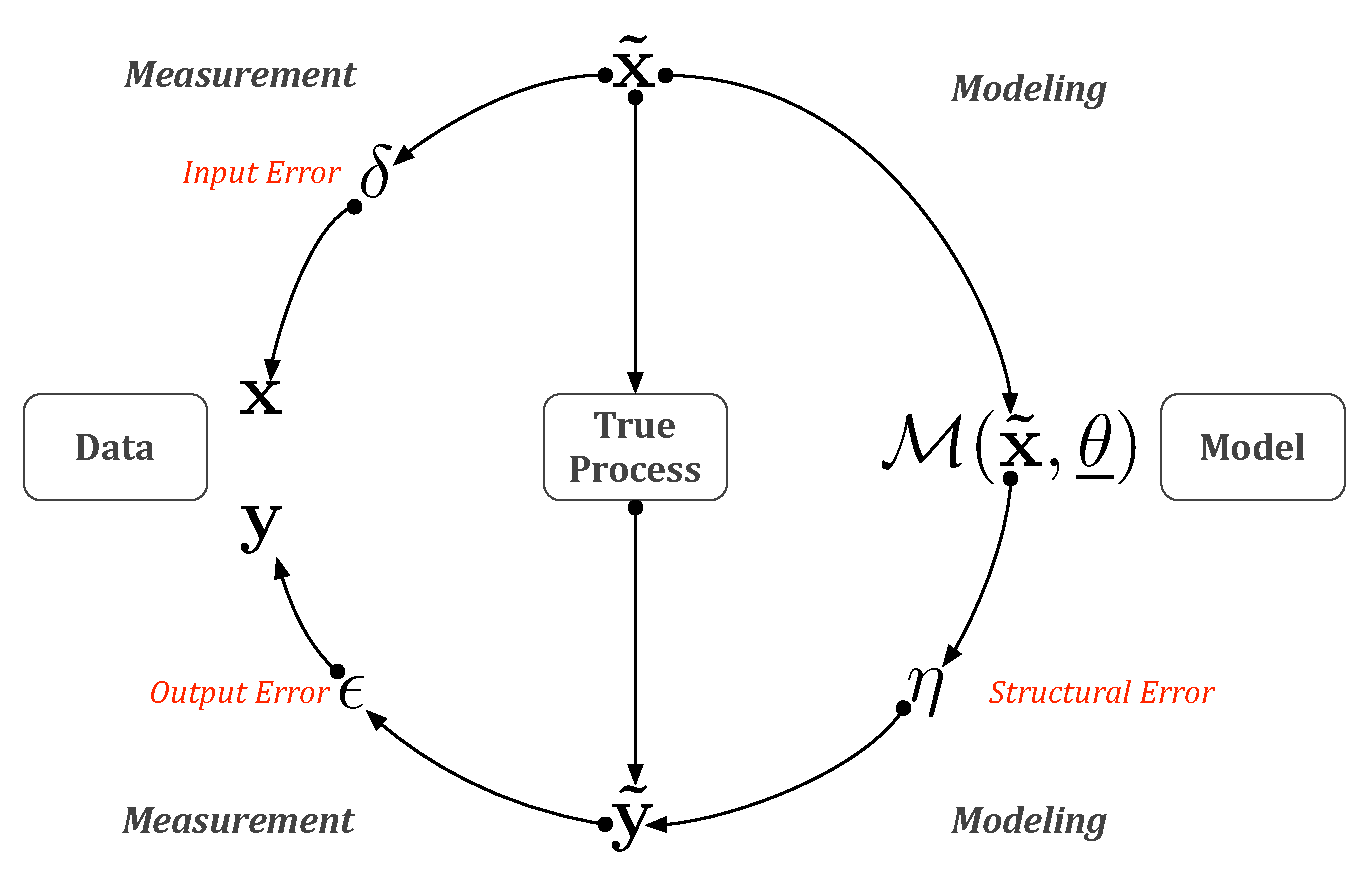
\includegraphics[width=0.55\textwidth]{HuardMailhot.pdf}
	\caption{Errors and their relation for Bayesian uncertainty analysis (adapted from \cite{HuardMailhot2006})}
	\label{fig:HuardMailhot}
\end{figure}

Input error refers to the difference between the true input $\mathbf{\tilde{x}}$ and the measured input $\mathbf{x}$. 
The measured input is limited by the imperfection of the measurement device. 
In the context of separate effect test, the input is the imposed initial and boundary conditions of the experiment. 
These conditions drive the system response during the test and they are measured with finite precision. 
Because the test conditions differ even within the same facility, these errors has to be taken into account for robust parameter estimation.

Output error is analogous to the input error described above. 
It is the difference between the true output $\mathbf{\tilde{y}}$ and the measured output $\mathbf{y}$. 
It is the system response for the imposed boundary conditions. 

Structural error is defined as the difference between model results and the true output $\mathbf{\tilde{y}}$. 
Modeling process relates the input to the output via a model parametrized with $\underline{\theta}$. 
By definition of model, even with a perfect set of parameters (which in principle, are also unknown, uncertain), model will still be inadequate. 
There are processes which are not taken into account either because lack of knowledge, fallacy in the hypothesis or even error in the numerical solution. 
As shown in \cite{KennedyOHagan2001}, not taking into account structural error during calibration biases the parameter estimates and reduces the model predictive capabilities.

The treatment of input and output errors belong to experimental data analysis and most of the time is straightforward. 
However, there is no standard approach to the model structural error. 
The structural error can be expected to show bias (due to incorrect or excluded process) as well as to be correlated in time and space, depending on the nature of problem. 
Several possibilities are available to model this error \cite{Simoen2013, Schoups2010}. 
In this context, an additional strength of Bayesian framework is that the plausibility of different error models can be checked and compared via their evidence as shown in \cite{Beck2010}.

In general, the above error model can be written as follows, independently of their forms:
\begin{equation}
\begin{array}{lrcr} 
	\text{Input} 	& p(\delta)	 	& \iff & p(\mathbf{x} \mid \mathbf{\tilde{x}}) \\ 
	\text{Output} 	& p(\epsilon) 	& \iff & p(\mathbf{y} \mid \mathbf{\tilde{y}}) \\
	\text{Structure}	& p(\eta) 		& \iff & p(\mathbf{\tilde{y}} \mid \mathbf{\tilde{x}}, \underline{\theta}, \mathcal{M}) 
\end{array}
\nonumber
\end{equation}
Note that the structural error model is conditioned on a specific model class $\mathcal{M}$ that defines its parametrization. 
To obtain the posterior distribution of the parameters based on their priors and conditioned on the data (both output and input) and specific model class, Bayes' theorem is applied,
\begin{equation}
\begin{array}{rcl} 
	p(\underline{\theta} \mid \mathbf{y}, \mathbf{x}, \mathcal{M} )	& = & \int \int p(\underline{\theta}, \mathbf{\tilde{y}}, \mathbf{\tilde{x}} \mid \mathbf{x}, \mathbf{y}, \mathcal{M} ) \: d\mathbf{\tilde{x}} d\mathbf{\tilde{y}} \\ 
		& = & \int \int p(\mathbf{x} \mid \mathbf{\tilde{x}}) \cdot p(\mathbf{y} \mid \mathbf{\tilde{y}}) \cdot p(\mathbf{\tilde{y}} \mid \mathbf{\tilde{x}}, \underline{\theta}, \mathcal{M} ) \cdot p(\mathbf{\tilde{x}}) \cdot \frac{p(\underline{\theta} \mid \mathcal{M})}{p(\mathbf{x}, \mathbf{y})} \: d\mathbf{\tilde{x}} d\mathbf{\tilde{y}}
\end{array}
\nonumber
\end{equation}
Where the posterior is condiioned on the observed data and model class $\mathcal{M}$. 
The integration is carried out to marginalize the joint distribution. 
To characterize the posterior distribution, Monte Carlo simulation is usually performed. 
One of the popular approach is to use Markov Chain Monte Carlo (MCMC) simulation to generate sample representative of the posterior.

%In essence, it is solving a traditional calibration problem. However as opposed to deterministic approach where the goal is to obtain single solution of optimum parameters, in Bayesian framework the effort is to explore the probability space to determine the uncertainty in the unknown given the observed data. Because sources of uncertainty can be modeled probabilistically, the inadequacy of the model can be also be modeled complementing the parametric uncertainty analysis as suggested in \cite{KennedyOHagan2001}. All of these avoid the risk of overfitting the parameters into a specific data set and cannot be applied for another.
%
%There are several key ideas of Bayesian framework that fit nicely into the uncertainty analysis of physical model in T-H system codes \cite{Beck2010}. They have both philosophical and practical points. First, the probability defining a set model parameters or even a model class, is viewed as a degree of confidence, as opposed to the frequency of occurrence. As the development of system code closure laws suggested, the sources of uncertainty are indeed due to lack of knowledge in the modeling processes or the experimental data required to support them. Models uncertainty quantification then means the quantification of state of knowledge in the models.
%
%Second, the probabilistic models can be update. This is the essence of Bayes' theorem \cite{Bayes}. The subsequent analysis will indeed be dependent to the available data and probabilistic model we choose to. If 
%
%Third and final, the updated posterior probability of parameter conditioned on the available data is a probabilistic statement combining all the available information at the analyst's hands: data and his own assumption. During \emph{forecasting}, where the code is used to simulate condition where there is no available data, this posterior is an important part of uncertainty analysis. They can be propagated to obtain robust prediction of the results along with their uncertainties.

\subsection{Context}  

Although the steps taken in this research can be applicable to any system code physical model calibration and validation, the attention will be focused on the models of particular importance during reflooding, the so-called Post-CHF flow regimes. 
The reasons for this emphasis are:
\begin{enumerate}
	\item Reflooding is an important part in the simulation of nuclear power plant transient during LOCA. 
	Modeling reflooding determines the appropriate representation of the dynamics of heat transfer phenomena during the effort to rewet an uncovered core. 
	Of paramount interest is to estimate the time the rod can be expected to be rewet as well as the maximum temperature reached prior to rewet. 
	Reflood is a transient with highly coupled hydrodynamic-heat transfer effects and it challenges the assumption made on the implemented closure laws. 
	Indeed, several Separate Effect Test (SET) reflood programs existed and were designed to validate reflood models in system code. 
	Unfortunately, no orchestrated effort so far to consolidate the generated data in general and into TRACE code in particular.
	\item The models are adequately complex. 
	It is complex that 5 flow regimes are involved in a single phenomena. 
	But as the source of data is from reflooding separate effect test facilities (SETFs), system effect can be excluded and analysis can be concentrated on limited set of models. 
	In fact, as already pointed out, reflood SETFs are designed to validate (and calibrate) reflood models in sytem codes.
	\item Additional data from another reflooding facilities are also available, including data obtained from series of experiments at the Neptun facility conducted at Paul Scherrer Institut during the 1990s, as well as data from experiments at the PERICLES facility conducted by CEA.
	\item It is the model considered in PREMIUM benchmark, thus there is possibility to compare the results of this research with the results of the other participants.
\end{enumerate}

%\subsection{Proposed Framework}
%
%
%
%In this research, uncertainty is viewed as a state of lack of knowledge. Thus the natural way of modeling uncertainty viewed in that manner is probabilistically in Bayesian sense; a measure of degree of belief. Subjectivity and objectivity in statistical treatment, indeed in science and engineering, are subject of long on-going controversy. The position we take on this issues follows the framework we chose, that it the analysis will have it's subjective elements. It is not necessarily mean as the effort is easier. On the contrary the main challenge is to be transparent and try to validate them. 
%    
%But one can certainly go beyond parameter estimation setting. Often 
%
%The proposed 
%
%Bayesian approach on parameter quantification
%
%There are 3 main steps in conducting Bayesian calibration of a model:
%
%\begin{enumerate}
%	\item It is the problem posed in the aforementioned PREMIUM benchmark. This benchmark provides an opportunity to obtain SETF
%	\item The problem is complex enough without being too complex. It is complex due to 5 flow regimes changes are involved in a single transient. But based on the experimental data from Separate Effect Test setup, the system and scaling effect can be minimized. Thus, concentration can really be put on less number the relevant correlations.
%	\item The reflooding is an important transient in the simulation of nuclear power plant. Such transient with highly coupled hydrodynamic-heat transfer effect challenges the assumption made on the closure laws development by the code developers. Quantification of uncertainty of their parameters will uncover deficiency in the modeling or requirement for additional data.
%	
%\end{enumerate}
 
%\subsubsection{System Identification}
%
%System identification
%
%\subsubsection{Constructing Data Model}
%
%\subsubsection{Constructing Prior Process}
%
%\newpage

\newpage
\section{Premiers résultats /  {\large\textit{First results}}: \textcolor{blue}{(1-2 pages)}}

%\subsection{TRACE Model of FEBA Test Section}

\subsection{Bayesian Calibration of a Turbulence Model}

As an illustrative example and to familiarize with the main idea of Bayesian framework and its method, simple case of physical model calibration were carried out during the first year. Here the RNG k-epsilon turbulence model (parametrized by 7 parameters) is calibrated using measurement data from backstep flow experiment \cite{Kasagi1995}. The turbulence model is implemented in the OpenFOAM framework where the backstep flow simulation model is part of the OpenFOAM validation case.

The first step in statistical calibration is to develop a stochastic error model that probabilistically relates measured data and simulation results. There are two stochastic error models considered in the present analysis, it is either assumed to be independent or spatially correlated with an exponential form of correlation (with correlation length scale to be estimated). Then Markov Chain Monte Carlo simulation were carried out to characterize the posterior of the parameter conditioned on the data.

The likelihood (error function) is formulated in line with the procedure given in \cite{Cheung2011}. Here as opposed to approach given by \cite{KennedyOHagan2001}, the multiplicative form discrepancy error was assumed such that no-slip boundary condition is retained. The discrepancy error was assumed to be Gaussian with mean$=1$ and standard deviation to be estimated.
\begin{equation}
\text{prob}(\{D\} | \vec{\theta}, M_j) = \frac{1}{\sqrt{((2\pi)^2 \times|K|)}} \text{exp} \left[ - \frac{(d-y)^T K^{-1} (d-y)}{2} \right]
\end{equation}
Where the $d$ is the measured velocity data, $y$ is the simulation results with a given set of parameters, and $K$ is the covariance matrix which depends on the model structure $M_j$. For $j=1$, $K = Ke + Ki$ (measurement and model discrepancy independent variance), while for $j=2$, $K = Ke + Kc$ (measurement and model discrepancy correlated variance).

This resulted in 8 parameters for $M_1$ and 9 parameters for $M_2$ to be calibrated. The priors are set to be uniform and independent with the mean for the turbulence model parameters corresponds to the default values in OpenFOAM and with $\pm50\%$ upper and lower bound values for each parameter. 1000 samples (1000 simulation runs) from the posterior is then taken using Markov Chain Monte Carlo algorithm implemented in Matlab \cite{Haario2006}. The priors and the results are tabulated in Table~\ref{tab:BoundsOfUniformPDFs} and Table~\ref{tab:StatMCMCCorr}, respectively, while the marginal posterior distribution is given in Figure for the 9 parameters model.
\begin{table}[htbp]
	\centering
		\caption{Bounds of Uniform PDFs}
		\begin{tabular}{l l l l l l}
			\hline \hline
												&	Parameter										& Initial 	& Lower			& Upper 		\\
			\hline
												& $C_\mu$											& $0.08450$ & $0.04225$ & $0.12675$ \\
												& $C_1$												& $1.42000$ & $0.71000$ & $2.13000$ \\
										  	& $C_2$												& $1.68000$ & $0.84000$ & $2.52000$ \\
			RNG k-$\epsilon$ 	& $\sigma_k$									& $0.71942$ & $0.35971$ & $1.07913$ \\
										  	& $\sigma_\epsilon$					  & $0.71942$ & $0.35971$ & $1.07913$ \\
										  	& $\eta_0$										& $4.38000$ & $2.19000$ & $6.57000$ \\
										  	& $\beta$							   			& $0.01200$ & $0.00600$ & $0.01800$ \\
			M1 (Independent)	& $\sigma_{\text{mod}}$				& $0.10000$ & $0.00000$ & $0.20000$ \\
			M2 (Correlated)		& $\sigma_{\text{mod}}$				& $0.10000$ & $0.00000$ & $0.20000$ \\
										  	& $\text{log}(\alpha)$				& $1.00000$ & $0.00000$ & $2.00000$ \\
			\hline
		\end{tabular}
	\label{tab:BoundsOfUniformPDFs}
\end{table}

\begin{table}[htbp]
	\centering
	    \caption{Statistics of MCMC samples of Correlated Model}
		\begin{tabular}{l l l l}
			\hline \hline
			Parameter										& mean 				& std.deviation			& MC Error 		\\
			\hline
			$C_\mu$											& $0.061714$	& $0.0060212$ 			& $0.0013311$ \\
			$C_1$												& $1.43980$	 	& $0.026246$ 				& $0.0047692 $ \\
			$C_2$												& $1.8468$ 		&	$0.10874$ 				& $0.023902$ \\
			$\sigma_k$									& $0.51179$ 	& $0.07683$ 				& $0.017243$ \\
			$\sigma_\epsilon$						& $0.81953$ 	& $0.01831$ 				& $0.0039055$ \\
			$\eta_0$										& $5.4496$ 		& $0.24451$ 				& $0.055019$ \\
			$\beta$							   			& $0.0095692$ & $0.00049043$ 			& $9.8941 \times 10^{-5}$ \\
			$\sigma_{\text{mod}}$				& $0.14952$ 	& $0.0072768$ 			& $0.0015929$ \\
			$\text{log}(\alpha)$				& $0.79485$ 	& $0.045782$ 				& $0.0099883$ \\       
			\hline
		\end{tabular}
	\label{tab:StatMCMCCorr}
\end{table}

\begin{figure}[htbp]
	\centering
	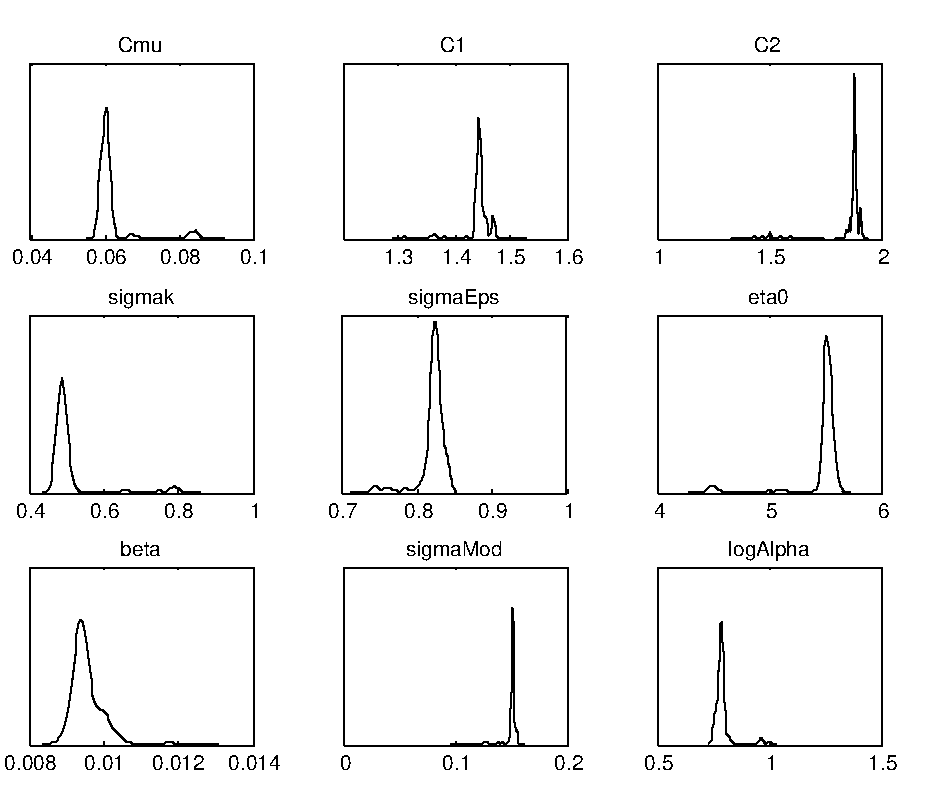
\includegraphics[width=0.9\textwidth]{ParamEstCorrDRAM.pdf}
	\caption{Marginal Posterior PDFs for Model Parameters}
	\label{fig:MarginalPosteriorPDFsForModelParameters}
\end{figure}
As can be seen, all the parameters are informed by the data. The uncertainties of the parameter obtained from the posterior can then be propagated to obtain robust prediction in other quantities (\textit{e.g.,} the wall shear stress). However it was not checked the robustness of the parameter estimation using another data sets. 

This exercise revealed some considerations in applying the Bayesian framework to calibrate TRACE reflood model with the data from reflood experiments:
\begin{enumerate}
	\item The reflood process is inherently transient in nature, so in addition to measurement on several locations, the data will also be in time series. This need to be considered in deriving error models especially if there is correlation structure both in space and time assumed.
	\item Incorporating several type of available data. In some facilities, several other quantities other than cladding temperature were also measured, including for example, pressure drop and void fraction. These call for several goodness-of-fit measures between data and model to be considered at once. Even if the importance of these additional data is less than clad temperature, they nevertheless contains additional information of reflood process.
	\item The boundary conditions in reflood experiment are dynamic in nature, the imposed power as well as the injected water temperature is time-dependent. Their uncertainties should also be taken into account.
	\item Parameters that need to be calibrated in TRACE reflood model are not part of the user input specification. Some were already hard-coded with values from a calibration with a data from a facility (without any statement of their uncertainties). Some modifications in the source code are required to accommodate sensitivity and uncertainty analysis of TRACE.
	\item Aggregating the uncertainty estimation of parameters of reflood model from a facility with another might not be straightforward. Although each reflood experiment in different facility basically experimented a reflood process in a rod bundle, specificities exist and might bias the results from each.
	\item Related to above concern, the statistical parameter estimation of reflood model in TRACE might not be identifiable with the available data from a facility, thus the result is sensitive to a condition in a given facility and by no mean unique.
\end{enumerate}

\newpage
\section{Planification future (plan de travail) /  {\large\textit{Future planning (scheme of work)}}:}

The proposed research plan, with emphasized placed on bottom reflood model and TRACE code, is expected to involve the following phases:
\begin{enumerate}
    \item First, comprehensive review of TRACE closure laws related to reflood phenomena. Most are part of the post-CHF closure package, which includes interfacial drag, wall drag, interfacial heat transfer, and wall heat transfer models or correlations. The goal is to obtain understanding how reflood is conceptualized in TRACE, and along with it how the models are parametrized. This will result in list of parameters that is perceived to be important in reflood simulation.
    \item Second, as these parameters are often not part of user specification and hard-coded in TRACE, modification of TRACE is required for it to accomodate sensitivity and uncertainty analyses. The goal here is to externalize important parameters hard-coded in TRACE, thus make them available for user to modify for each run.  
    \item Third, based on FEBA separate effect test facility, global sensitivity analysis of assumed important parameters (including the boundary and initial conditions) is carried out for the available type of measured data. In Bayesian framework, sensitivity analysis is an important for the purpose of system identification. In essence, if a measured value is insensitive to a (perceived) important parameter, then the uncertainty of this parameter cannot be inferred from this particular data. Excluding them prior to posterior sampling will save computational time or even reveal modeling error.
    \item Fourth, based on several error models that can be assumed, posterior sampling is carried out to obtain the uncertainty in the parameters. The posterior sampling is performed via Markov Chain Monte Carlo (MCMC) illustrated in the example above. Further analysis for selecting (or averaging) the most plausible error model is done in this phase.
    \item Next is the validation phase where the uncertainties obtained will be propagated in ``forecasting'' setting, using different data sets than the one used to derive the uncertainty of the model parameter. 
    \item Fifth, the uncertainties of parameters obtained from two different facilities  need to be consistently combined while taking into account the facilities specificity and different range of experimental conditions. This phase involves a repetition of phase 3-5 but based on different facility (\textit{e.g.}, PERICLES). 
    \item Finally, the results of combined uncertainties estimates need to be validated yet against another facility (\textit{e.g.}, NEPTUN). The goal here is to investigate if indeed experimental data from different reflood SETFs can be consolidated into the current implementation of reflood model in TRACE to increase its predictive capability in simulating reflood process.
\end{enumerate}

Basically for a given of reflood facility, the routine procedure would be: sensitivity analysis - uncertainty (backward) analysis for parametric calibration - uncertainty (forward) analysis for validation. The analyses at first are carried out separately for each reflood facilities. At the latter stage, however, the results will be consolidated where the uncertainty information of reflood physical model based on the data from various facilities are combined together in a consistent way, minimizing the specificity of the facilities and/or the experimental conditions.

Based on the phases identified above, a preliminary schedule for the 3-year dissertation work is proposed as follows:

\begin{enumerate}
    \item \textbf{Task 1 (3 months)}
        \begin{itemize}
            \item List the important parameters in TRACE that are perceived to be important for reflood simulation in SETF.
            \item Externalize these parameters such that it can be specified in an input deck for the purpose of sensitivity and uncertainty analyses 
        \end{itemize}
    \item \textbf{Task 2 (3 months)}
        \begin{itemize}
            \item Test the modified TRACE for global sensitivity analysis.
            \item Finalize the development of TRACE model for FEBA test facility.
            \item Carried out global uncertainty analysis of FEBA test facility.
        \end{itemize}
   \item \textbf{Task 3 (10 months)}
        \begin{itemize}
            \item Develop various plausible error models for input, output, and structural errors applicable for reflood model calibration. The nature of available data needs to be taken into account, that they are time series of measured values taken from different location. Possibility to incorporate information from different type of data (\textit{e.g.,} temperature and void fraction) need also to be considered.   
            \item Develop or adapt available MCMC sampling algorithm that is efficient, can be parallelized, with informative diagnostics. 
            \item Carried out MCMC sampling based on each of the plausible structure of error models to characterize the uncertainty in the parameters conditioned on the data.
            \item Select the more plausible model based on the evaluation of the evidence of these models.
            \item If the reflood simulation proved to be too computationally demanding, develop a surrogate models to assist the calibration procedure.
         \end{itemize}
   \item \textbf{Task 4 (1 month)}. Validation of the obtain uncertainty estimates by propagating them for another data set within the same facility (FEBA).
   \item \textbf{Task 5 (10 months)}. In principle, repeat most of the previous four tasks for other reflood facilities (\textit{e.g.,} PERICLES and ACHILLES) to obtain the uncertainties in the important parameters.   
   \item \textbf{Task 3 (6 months)}: Consolidation and Validation
        \begin{itemize}
            \item Develop procedure to consolidate parameter estimation of reflood models based on two/three different reflood facilities.
            \item Validation of the consolidated uncertainty estimates of the parameters by propagating them in the simulation of reflood using data set from another facility (\textit{e.g.,} NEPTUN).
        \end{itemize}
   \item \textbf{Thesis write-up (3 months)}: 
\end{enumerate}

%The research can be broad
%
%\subsection{Phase I: Literature Survey and Familiarization with a reflood SETF Model}
%At this phase, it was agreed that the problem of quantifying uncertainty in a specific physical models built-in in system codes can be done by using Bayesian framework. Under this framework, the uncertainty on a model parameters can be updated based on 
%
%\subsection{Phase II: Modification of TRACE}
%
%\subsection{Phase III: Sensitivity Analysis}
%
%At this phase the foreseen important

\newpage
\section{Divers /  {\large\textit{Miscellaneous}}}

\subsection{Eventuelles publications / {\small \textit{Publications}}}
\subsection{Présentation(s) orale(s) / {\small \textit{Oral presentation(s)}}}
\subsection{Cours suivis / {\small \textit{Courses attended}}}


\newpage
\section{Références /  {\large\textit{References}}}

\bibliographystyle{IEEEtran}
% No additional "reference" title please
\begingroup
\renewcommand{\section}[2]{}%
%\renewcommand{\chapter}[2]{}% for other classes
\bibliography{ResearchPlan}
\endgroup


\newpage
\section{Signatures}
Candidat(e)/\textit{Candidate}\hspace{8.3cm}...............................................\\

\noindent Directeur de thèse/\textit{Thesis director}\hspace{6.5cm}...............................................\\

\noindent Co-directeur de thèse/\textit{Thesis co-director}\hspace{5.5cm}...............................................\\
\noindent (Officiellement habilité / \textit{Officially authorized)}\\

\noindent Date du rapport/\textit{Date of report}\hspace{7cm}...............................................\\

\vspace{0.8cm}
\noindent Directeur du programme/\textit{Program director} \\

\noindent Signature: ......................................................\hspace{4cm}Date: ..........................................\\

\vspace{0.8cm}
\begin{center}
\textcolor{green}{A retourner à : EDPY – Station 3 – 1015 Lausanne\\
To be returned to : EDPY– Station 3 – 1015 Lausanne}
\end{center}
\end{document}  
